\chapter{Architecture}

Developed architecture / system design / implementation: 1/3

\begin{itemize}
\item start with a theoretical approach
\item describe the developed system/algorithm/method from a high-level point of view
\item go ahead in presenting your developments in more detail
\end{itemize}

\section{Sample Application}
For verifying that the \textit{Azure IoT Edge} software behaves correctly
with the given operating system, a sample application was developed. This
containerized sample application sends a randomly generated number to the
\textit{Edge Hub}.

The application features a \ac{HTTP} \ac{REST} \ac{API} for further automation.

\begin{table}[H]
    \centering
    \begin{tabular}{ p{0.33\textwidth} p{0.14\textwidth} p{0.45\textwidth}}
        \toprule
        \textbf{Container Name} & \textbf{Developer} & \textbf{Description} \\
        \midrule
        Edge Agent & Microsoft & Application for managing containers and deployments. \\
        Edge Hub & Microsoft & Gateway and buffer for sending messages to cloud services. \\
        Edge Metrics Collector & Microsoft & Application for collecting container logs, metrics and health data. \\
        SQL Server & Microsoft & Containerized instance of Microsoft's SQL server. \\
        sampleapp UI & Elias Frank & Web application for viewing telemetry data from the \ac{API}. \\
        sampleapp API & Elias Frank & \ac{REST} \ac{API} for retrieving telemetry locally for further automation. \\
        sampleapp Telemetry Service & Elias Frank & Background service for randomly generating telemetry. \\
        \bottomrule
    \end{tabular}
    \caption{Sample Application: List of containers}
\end{table}

\begin{table}[H]
    \centering
    \begin{tabular}{l l l l }
        \toprule
        \textbf{From} & \textbf{To} & \textbf{Port} & \textbf{Protocol} \\
        \midrule
        sampleapp Telemetry Service & Edge Hub & C & D \\
        sampleapp Telemetry Service & SQL Server & C & D \\
        Edge Metrics Collector & Edge Agent & 9000 & \ac{HTTP} \\
        Edge Metrics Collector & Edge Hub & 9000 & \ac{HTTP} \\
        Edge Metrics Collector & sampleapp API & 8080 & \ac{HTTP} \\
        Edge Metrics Collector & sampleapp Telemetry Service & 8080 & \ac{HTTP} \\
        \bottomrule
    \end{tabular}
    \caption{Sample Application: Communication table}
\end{table}


\begin{figure}[H]
    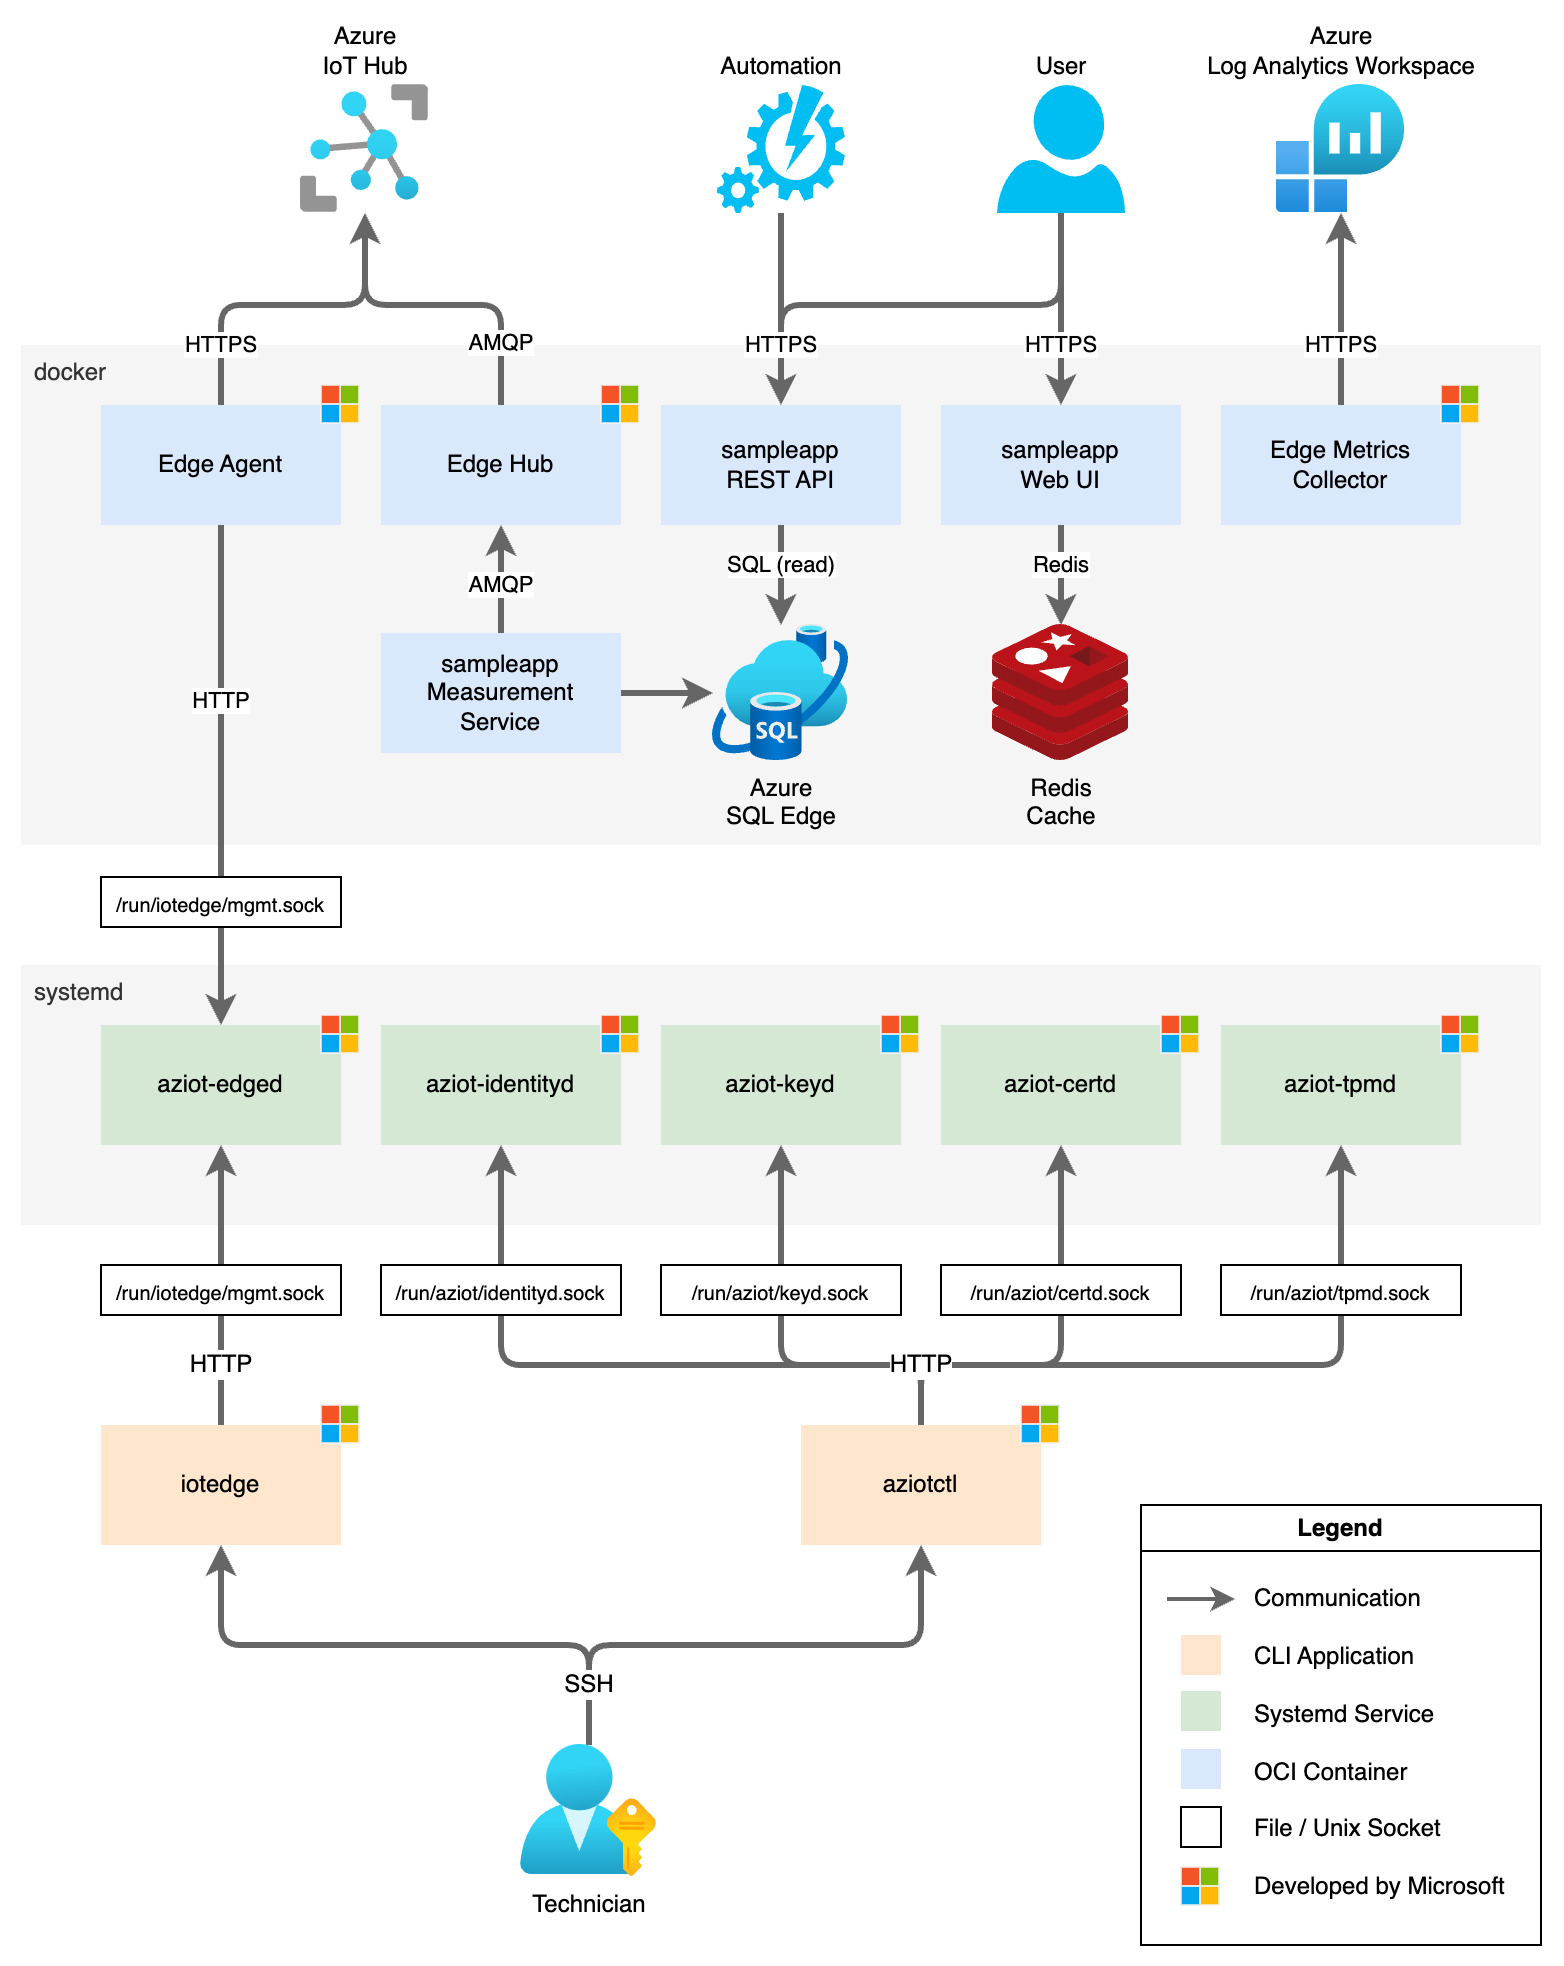
\includegraphics[width=\textwidth]{fig/sample-app-dataflow.drawio.png}
    \caption{Sample Application: Architecture Overview}
    \label{fig:sample-app-architecture}
\end{figure}

\section{Experiments}
\subsection{Image size}
When updating the operating system with an A/B failover model, the entire
image needs to be downloaded and written to a secondary partition. In this
\ac{OTA} scenario the size of the operating system image is critical.
For this experiment two sizes are relevant, when comparing operating systems.
Firstly, the actual size of the image that needs to be written to the partition.
Secondly, the size that the entire system takes up on the disk after booting.
\subsubsection{Transmitted image size}
\subsubsection{Size on disk}
The size on disk will be measured after the system has successfully booted
and started all \textit{Azure IoT Edge} services including the containerized
applications. To see if the containers have been successfully started,
Microsoft provides the command line interface \textit{iotedge}.
With the following command, it is possible to list all running containers.\\

\begin{lstlisting}[caption=Command to retrieve the status of all containers]
iotedge list
\end{lstlisting}
After all containers are running, it is possible to read out the disk utilization
with the \textit{df} command line interface. \cite{man-df}\\

\begin{lstlisting}[caption=Command to report file system space usage]
df -h
\end{lstlisting}
The value of the disk utilization excluding the \textit{/var} directory
can be used for comparing operating systems.



\subsection{Time to recover}
\subsection{Endurance}
